%\vita
\coverbio
\begin{tabular}{p{.3\textwidth}|p{.68\textwidth}}
\raisebox{-1.3\height}{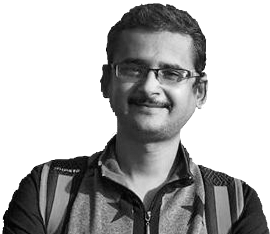
\includegraphics[width=.3\textwidth]{100-back/closeUp3.png}} &
\large{\textbf{Subhrendu Chattopadhyay} born in West Bengal, India. After completion of school education, he has completed the B.Tech from \emph{West Bengal University of Technology} (Now MAKAUT) in the area of
 \emph{Computer Science and Engineering} in 2010. He has completed M.Tech from the \emph{Department of Computer Science and Engineering}, \emph{Indian Institute of Technology Guwahati}, India in 2014, where he has continued working towards the PhD degree under the supervision of \textbf{Prof. Sukumar Nandi}. He has received \emph{TCS Research Scholar Fellowship} from Tata Consultancy Services, India for pursuing his PhD program. He has received best paper awards from \emph{IEEE ANTS 2013}, \emph{IEEE COMSNETS 2016} and best in session award from \emph{IEEE INFOCOM 2019}. His research interests include network architecture and management, wireless networks, distributed algorithms. He is interested to develop a cognitive network management architecture.}
\end{tabular}
\endcoverbio

